\documentclass[11pt]{article}
\usepackage[margin=1in]{geometry}
\usepackage[T1]{fontenc}
\usepackage{lmodern}
\usepackage{amsmath,amssymb,amsthm}
\usepackage{graphicx}
\usepackage{booktabs,array}
\usepackage[hidelinks]{hyperref}
\usepackage{microtype}
\usepackage{listings,xcolor,needspace}
\newcommand{\solution}{\par\medskip\noindent\textbf{Solution.}\enspace\ignorespaces}
\renewcommand{\arraystretch}{1.16}
\setlength{\parindent}{0pt}
\setlength{\parskip}{3pt}
\setlength{\emergencystretch}{1em}
\raggedbottom
\urlstyle{same}
\lstset{basicstyle=\ttfamily\footnotesize,columns=fullflexible,
  keepspaces=true,showstringspaces=false,breaklines=true,
  breakatwhitespace=false,tabsize=4,aboveskip=5pt,belowskip=8pt,
  keywordstyle=\color{black},commentstyle=\color{black},stringstyle=\color{black}}
\lstdefinestyle{output}{language={},basicstyle=\ttfamily\footnotesize}
\title{ELEC 576 / COMP 576\\[1ex]\large Assignment 0}
\author{Yunfei Xie (yx106)}
\date{September 15, 2026}
\begin{document}
\maketitle

\section*{\fbox{Task 1}}
\textbf{Question.}
Install Anaconda and confirm that it is working. In a terminal, run
\texttt{conda info} and paste the result into the report.

\solution
I installed Anaconda Distribution 2026.07-1 for Apple silicon and
activated its base environment. Both \texttt{conda list} and
\texttt{conda info} completed successfully. The terminal output from
\texttt{conda info} is
\lstinputlisting[style=output]{snippets/conda-info.txt}

\clearpage
\section*{\fbox{Task 2}}
\textbf{Question.}
Run all Python commands in the ``Linear Algebra Equivalents'' table in
\emph{NumPy for MATLAB Users}. Use IPython and paste the results into
the report. Any matrices may be used.

\solution
I ran all 82 rows of the linked table in an IPython kernel, including
the alternative commands listed within a row \cite{numpy}.
The inputs below use NumPy arrays. Array entries are displayed with up
to six decimal places; the calculations use full floating-point precision.
Each numbered entry follows the corresponding table row and includes
its code and captured output.

The table has a few syntax and behavior differences in the installed
versions. I show the errors from its older random-number and resampling
calls, followed by working calls. The relevant entries also explain
Boolean-mask shape, grid orientation, and sorting axes.

\subsection*{Shared inputs}
\noindent\texttt{In [2]:}
\lstinputlisting[language=Python]{snippets/task2-setup.py}
\par\noindent\begin{minipage}{\linewidth}
\noindent\texttt{Shared input values:}
\lstinputlisting[style=output]{snippets/task2-setup.txt}
\end{minipage}\par
The indexing examples use a larger array where needed. The matrix
\texttt{spd} is symmetric positive definite; its leading principal
minors are $6$, $26$, and $83$, so it is suitable for Cholesky
factorization and conjugate gradients.


\par\medskip\noindent\begin{minipage}{\linewidth}
\subsection*{2.1 Dimensions}
\noindent\texttt{In [3]:}
\lstinputlisting[language=Python]{snippets/task2-01.py}
\noindent\texttt{Output:}
\lstinputlisting[style=output]{snippets/task2-01.txt}
\end{minipage}\par

\par\medskip\noindent\begin{minipage}{\linewidth}
\subsection*{2.2 Number of elements}
\noindent\texttt{In [4]:}
\lstinputlisting[language=Python]{snippets/task2-02.py}
\noindent\texttt{Output:}
\lstinputlisting[style=output]{snippets/task2-02.txt}
\end{minipage}\par

\par\medskip\noindent\begin{minipage}{\linewidth}
\subsection*{2.3 Array shape}
\noindent\texttt{In [5]:}
\lstinputlisting[language=Python]{snippets/task2-03.py}
\noindent\texttt{Output:}
\lstinputlisting[style=output]{snippets/task2-03.txt}
\end{minipage}\par

\par\medskip\noindent\begin{minipage}{\linewidth}
\subsection*{2.4 Length of one axis}
\noindent\texttt{In [6]:}
\lstinputlisting[language=Python]{snippets/task2-04.py}
\noindent\texttt{Output:}
\lstinputlisting[style=output]{snippets/task2-04.txt}
\end{minipage}\par

\par\medskip\noindent\begin{minipage}{\linewidth}
\subsection*{2.5 Create an array}
\noindent\texttt{In [7]:}
\lstinputlisting[language=Python]{snippets/task2-05.py}
\noindent\texttt{Output:}
\lstinputlisting[style=output]{snippets/task2-05.txt}
\end{minipage}\par

\par\medskip\noindent\begin{minipage}{\linewidth}
\subsection*{2.6 Assemble blocks}
\noindent\texttt{In [8]:}
\lstinputlisting[language=Python]{snippets/task2-06.py}
\noindent\texttt{Output:}
\lstinputlisting[style=output]{snippets/task2-06.txt}
\end{minipage}\par

\par\medskip\noindent\begin{minipage}{\linewidth}
\subsection*{2.7 Last vector entry}
\noindent\texttt{In [9]:}
\lstinputlisting[language=Python]{snippets/task2-07.py}
\noindent\texttt{Output:}
\lstinputlisting[style=output]{snippets/task2-07.txt}
\end{minipage}\par

\par\medskip\noindent\begin{minipage}{\linewidth}
\subsection*{2.8 One matrix entry}
\noindent\texttt{In [10]:}
\lstinputlisting[language=Python]{snippets/task2-08.py}
\noindent\texttt{Output:}
\lstinputlisting[style=output]{snippets/task2-08.txt}
\end{minipage}\par

\par\medskip\noindent\begin{minipage}{\linewidth}
\subsection*{2.9 One row}
\noindent\texttt{In [11]:}
\lstinputlisting[language=Python]{snippets/task2-09.py}
\noindent\texttt{Output:}
\lstinputlisting[style=output]{snippets/task2-09.txt}
\end{minipage}\par

\par\medskip\noindent\begin{minipage}{\linewidth}
\subsection*{2.10 First five rows}
\noindent\texttt{In [12]:}
\lstinputlisting[language=Python]{snippets/task2-10.py}
\noindent\texttt{Output:}
\lstinputlisting[style=output]{snippets/task2-10.txt}
\end{minipage}\par

\par\medskip\noindent\begin{minipage}{\linewidth}
\subsection*{2.11 Last five rows}
\noindent\texttt{In [13]:}
\lstinputlisting[language=Python]{snippets/task2-11.py}
\noindent\texttt{Output:}
\lstinputlisting[style=output]{snippets/task2-11.txt}
\end{minipage}\par

\par\medskip\noindent\begin{minipage}{\linewidth}
\subsection*{2.12 A rectangular slice}
\noindent\texttt{In [14]:}
\lstinputlisting[language=Python]{snippets/task2-12.py}
\noindent\texttt{Output:}
\lstinputlisting[style=output]{snippets/task2-12.txt}
\end{minipage}\par

\par\medskip\noindent\begin{minipage}{\linewidth}
\subsection*{2.13 Selected rows and columns}
\noindent\texttt{In [15]:}
\lstinputlisting[language=Python]{snippets/task2-13.py}
\noindent\texttt{Output:}
\lstinputlisting[style=output]{snippets/task2-13.txt}
\end{minipage}\par

\par\medskip\noindent\begin{minipage}{\linewidth}
\subsection*{2.14 Rows 3 through 21 with a stride of two}
\noindent\texttt{In [16]:}
\lstinputlisting[language=Python]{snippets/task2-14.py}
\noindent\texttt{Output:}
\lstinputlisting[style=output]{snippets/task2-14.txt}
\end{minipage}\par

\par\medskip\noindent\begin{minipage}{\linewidth}
\subsection*{2.15 Every other row}
\noindent\texttt{In [17]:}
\lstinputlisting[language=Python]{snippets/task2-15.py}
\noindent\texttt{Output:}
\lstinputlisting[style=output]{snippets/task2-15.txt}
\end{minipage}\par

\par\medskip\noindent\begin{minipage}{\linewidth}
\subsection*{2.16 Reverse the rows}
\noindent\texttt{In [18]:}
\lstinputlisting[language=Python]{snippets/task2-16.py}
\noindent\texttt{Output:}
\lstinputlisting[style=output]{snippets/task2-16.txt}
\end{minipage}\par

\par\medskip\noindent\begin{minipage}{\linewidth}
\subsection*{2.17 Append the first row}
\noindent\texttt{In [19]:}
\lstinputlisting[language=Python]{snippets/task2-17.py}
\noindent\texttt{Output:}
\lstinputlisting[style=output]{snippets/task2-17.txt}
\end{minipage}\par

\par\medskip\noindent\begin{minipage}{\linewidth}
\subsection*{2.18 Transpose}
\noindent\texttt{In [20]:}
\lstinputlisting[language=Python]{snippets/task2-18.py}
\noindent\texttt{Output:}
\lstinputlisting[style=output]{snippets/task2-18.txt}
\end{minipage}\par

\par\medskip\noindent\begin{minipage}{\linewidth}
\subsection*{2.19 Conjugate transpose}
\noindent\texttt{In [21]:}
\lstinputlisting[language=Python]{snippets/task2-19.py}
\noindent\texttt{Output:}
\lstinputlisting[style=output]{snippets/task2-19.txt}
\end{minipage}\par

\par\medskip\noindent\begin{minipage}{\linewidth}
\subsection*{2.20 Matrix multiplication}
\noindent\texttt{In [22]:}
\lstinputlisting[language=Python]{snippets/task2-20.py}
\noindent\texttt{Output:}
\lstinputlisting[style=output]{snippets/task2-20.txt}
\end{minipage}\par

\par\medskip\noindent\begin{minipage}{\linewidth}
\subsection*{2.21 Elementwise multiplication}
\noindent\texttt{In [23]:}
\lstinputlisting[language=Python]{snippets/task2-21.py}
\noindent\texttt{Output:}
\lstinputlisting[style=output]{snippets/task2-21.txt}
\end{minipage}\par

\par\medskip\noindent\begin{minipage}{\linewidth}
\subsection*{2.22 Elementwise division}
\noindent\texttt{In [24]:}
\lstinputlisting[language=Python]{snippets/task2-22.py}
\noindent\texttt{Output:}
\lstinputlisting[style=output]{snippets/task2-22.txt}
\end{minipage}\par

\par\medskip\noindent\begin{minipage}{\linewidth}
\subsection*{2.23 Elementwise powers}
\noindent\texttt{In [25]:}
\lstinputlisting[language=Python]{snippets/task2-23.py}
\noindent\texttt{Output:}
\lstinputlisting[style=output]{snippets/task2-23.txt}
\end{minipage}\par

\par\medskip\noindent\begin{minipage}{\linewidth}
\subsection*{2.24 A Boolean comparison}
\noindent\texttt{In [26]:}
\lstinputlisting[language=Python]{snippets/task2-24.py}
\noindent\texttt{Output:}
\lstinputlisting[style=output]{snippets/task2-24.txt}
\end{minipage}\par

\par\medskip\noindent\begin{minipage}{\linewidth}
\subsection*{2.25 Indices satisfying a condition}
\noindent\texttt{In [27]:}
\lstinputlisting[language=Python]{snippets/task2-25.py}
\noindent\texttt{Output:}
\lstinputlisting[style=output]{snippets/task2-25.txt}
\end{minipage}\par

\par\medskip\noindent\begin{minipage}{\linewidth}
\subsection*{2.26 Select columns using index positions}
\noindent\texttt{In [28]:}
\lstinputlisting[language=Python]{snippets/task2-26.py}
\noindent\texttt{Output:}
\lstinputlisting[style=output]{snippets/task2-26.txt}
\end{minipage}\par

\par\medskip\noindent\begin{minipage}{\linewidth}
\subsection*{2.27 Select columns using a Boolean mask}
The first call uses a one-dimensional vector. For an actual two-dimensional column vector, ravel() gives a one-dimensional column mask.

\noindent\texttt{In [29]:}
\lstinputlisting[language=Python]{snippets/task2-27.py}
\noindent\texttt{Output:}
\lstinputlisting[style=output]{snippets/task2-27.txt}
\end{minipage}\par

\par\medskip\noindent\begin{minipage}{\linewidth}
\subsection*{2.28 Replace entries below a threshold}
\noindent\texttt{In [30]:}
\lstinputlisting[language=Python]{snippets/task2-28.py}
\noindent\texttt{Output:}
\lstinputlisting[style=output]{snippets/task2-28.txt}
\end{minipage}\par

\par\medskip\noindent\begin{minipage}{\linewidth}
\subsection*{2.29 Multiply by a strict Boolean mask}
The entry equal to 0.5 becomes zero here. It remains 0.5 in the previous example because that assignment tests a < 0.5.

\noindent\texttt{In [31]:}
\lstinputlisting[language=Python]{snippets/task2-29.py}
\noindent\texttt{Output:}
\lstinputlisting[style=output]{snippets/task2-29.txt}
\end{minipage}\par

\par\medskip\noindent\begin{minipage}{\linewidth}
\subsection*{2.30 Fill an array}
\noindent\texttt{In [32]:}
\lstinputlisting[language=Python]{snippets/task2-30.py}
\noindent\texttt{Output:}
\lstinputlisting[style=output]{snippets/task2-30.txt}
\end{minipage}\par

\par\medskip\noindent\begin{minipage}{\linewidth}
\subsection*{2.31 Copy an array}
Changing the copy leaves x unchanged.

\noindent\texttt{In [33]:}
\lstinputlisting[language=Python]{snippets/task2-31.py}
\noindent\texttt{Output:}
\lstinputlisting[style=output]{snippets/task2-31.txt}
\end{minipage}\par

\par\medskip\noindent\begin{minipage}{\linewidth}
\subsection*{2.32 Copy a row}
\noindent\texttt{In [34]:}
\lstinputlisting[language=Python]{snippets/task2-32.py}
\noindent\texttt{Output:}
\lstinputlisting[style=output]{snippets/task2-32.txt}
\end{minipage}\par

\par\medskip\noindent\begin{minipage}{\linewidth}
\subsection*{2.33 Flatten an array}
The default traversal reads rows first. The F option reads columns first, matching MATLAB linear indexing.

\noindent\texttt{In [35]:}
\lstinputlisting[language=Python]{snippets/task2-33.py}
\noindent\texttt{Output:}
\lstinputlisting[style=output]{snippets/task2-33.txt}
\end{minipage}\par

\par\medskip\noindent\begin{minipage}{\linewidth}
\subsection*{2.34 The values 1 through 10}
\noindent\texttt{In [36]:}
\lstinputlisting[language=Python]{snippets/task2-34.py}
\noindent\texttt{Output:}
\lstinputlisting[style=output]{snippets/task2-34.txt}
\end{minipage}\par

\par\medskip\noindent\begin{minipage}{\linewidth}
\subsection*{2.35 The values 0 through 9}
\noindent\texttt{In [37]:}
\lstinputlisting[language=Python]{snippets/task2-35.py}
\noindent\texttt{Output:}
\lstinputlisting[style=output]{snippets/task2-35.txt}
\end{minipage}\par

\par\medskip\noindent\begin{minipage}{\linewidth}
\subsection*{2.36 A column vector}
\noindent\texttt{In [38]:}
\lstinputlisting[language=Python]{snippets/task2-36.py}
\noindent\texttt{Output:}
\lstinputlisting[style=output]{snippets/task2-36.txt}
\end{minipage}\par

\par\medskip\noindent\begin{minipage}{\linewidth}
\subsection*{2.37 A zero matrix}
\noindent\texttt{In [39]:}
\lstinputlisting[language=Python]{snippets/task2-37.py}
\noindent\texttt{Output:}
\lstinputlisting[style=output]{snippets/task2-37.txt}
\end{minipage}\par

\par\medskip\noindent\begin{minipage}{\linewidth}
\subsection*{2.38 A three-dimensional zero array}
\noindent\texttt{In [40]:}
\lstinputlisting[language=Python]{snippets/task2-38.py}
\noindent\texttt{Output:}
\lstinputlisting[style=output]{snippets/task2-38.txt}
\end{minipage}\par

\par\medskip\noindent\begin{minipage}{\linewidth}
\subsection*{2.39 An array of ones}
\noindent\texttt{In [41]:}
\lstinputlisting[language=Python]{snippets/task2-39.py}
\noindent\texttt{Output:}
\lstinputlisting[style=output]{snippets/task2-39.txt}
\end{minipage}\par

\par\medskip\noindent\begin{minipage}{\linewidth}
\subsection*{2.40 An identity matrix}
\noindent\texttt{In [42]:}
\lstinputlisting[language=Python]{snippets/task2-40.py}
\noindent\texttt{Output:}
\lstinputlisting[style=output]{snippets/task2-40.txt}
\end{minipage}\par

\par\medskip\noindent\begin{minipage}{\linewidth}
\subsection*{2.41 Read a diagonal}
\noindent\texttt{In [43]:}
\lstinputlisting[language=Python]{snippets/task2-41.py}
\noindent\texttt{Output:}
\lstinputlisting[style=output]{snippets/task2-41.txt}
\end{minipage}\par

\par\medskip\noindent\begin{minipage}{\linewidth}
\subsection*{2.42 Construct a diagonal matrix}
\noindent\texttt{In [44]:}
\lstinputlisting[language=Python]{snippets/task2-42.py}
\noindent\texttt{Output:}
\lstinputlisting[style=output]{snippets/task2-42.txt}
\end{minipage}\par

\par\medskip\noindent\begin{minipage}{\linewidth}
\subsection*{2.43 Random values with a fixed seed}
The older call in the table passes a tuple to rand, which expects separate dimension arguments. The corrected call is random.rand(3, 4). The two generators use different random streams.

\noindent\texttt{In [45]:}
\lstinputlisting[language=Python]{snippets/task2-43.py}
\noindent\texttt{Output:}
\lstinputlisting[style=output]{snippets/task2-43.txt}
\end{minipage}\par

\par\medskip\noindent\begin{minipage}{\linewidth}
\subsection*{2.44 Evenly spaced values}
\noindent\texttt{In [46]:}
\lstinputlisting[language=Python]{snippets/task2-44.py}
\noindent\texttt{Output:}
\lstinputlisting[style=output]{snippets/task2-44.txt}
\end{minipage}\par

\par\medskip\noindent\begin{minipage}{\linewidth}
\subsection*{2.45 Dense coordinate grids}
mgrid returns arrays shaped (9, 6); meshgrid uses (6, 9) with its default xy indexing.

\noindent\texttt{In [47]:}
\lstinputlisting[language=Python]{snippets/task2-45.py}
\noindent\texttt{Output:}
\lstinputlisting[style=output]{snippets/task2-45.txt}
\end{minipage}\par

\par\medskip\noindent\begin{minipage}{\linewidth}
\subsection*{2.46 Open coordinate grids}
The table omits the closing parenthesis in its ix\_ call. The calls here include the np namespace and the missing parenthesis.

\noindent\texttt{In [48]:}
\lstinputlisting[language=Python]{snippets/task2-46.py}
\noindent\texttt{Output:}
\lstinputlisting[style=output]{snippets/task2-46.txt}
\end{minipage}\par

\par\medskip\noindent\begin{minipage}{\linewidth}
\subsection*{2.47 An irregular dense grid}
\noindent\texttt{In [49]:}
\lstinputlisting[language=Python]{snippets/task2-47.py}
\noindent\texttt{Output:}
\lstinputlisting[style=output]{snippets/task2-47.txt}
\end{minipage}\par

\par\medskip\noindent\begin{minipage}{\linewidth}
\subsection*{2.48 An irregular open grid}
\noindent\texttt{In [50]:}
\lstinputlisting[language=Python]{snippets/task2-48.py}
\noindent\texttt{Output:}
\lstinputlisting[style=output]{snippets/task2-48.txt}
\end{minipage}\par

\par\medskip\noindent\begin{minipage}{\linewidth}
\subsection*{2.49 Repeat a matrix}
\noindent\texttt{In [51]:}
\lstinputlisting[language=Python]{snippets/task2-49.py}
\noindent\texttt{Output:}
\lstinputlisting[style=output]{snippets/task2-49.txt}
\end{minipage}\par

\par\medskip\noindent\begin{minipage}{\linewidth}
\subsection*{2.50 Join columns}
\noindent\texttt{In [52]:}
\lstinputlisting[language=Python]{snippets/task2-50.py}
\noindent\texttt{Output:}
\lstinputlisting[style=output]{snippets/task2-50.txt}
\end{minipage}\par

\par\medskip\noindent\begin{minipage}{\linewidth}
\subsection*{2.51 Join rows}
\noindent\texttt{In [53]:}
\lstinputlisting[language=Python]{snippets/task2-51.py}
\noindent\texttt{Output:}
\lstinputlisting[style=output]{snippets/task2-51.txt}
\end{minipage}\par

\par\medskip\noindent\begin{minipage}{\linewidth}
\subsection*{2.52 Maximum over all entries}
nanmax ignores the inserted NaN, while max propagates it.

\noindent\texttt{In [54]:}
\lstinputlisting[language=Python]{snippets/task2-52.py}
\noindent\texttt{Output:}
\lstinputlisting[style=output]{snippets/task2-52.txt}
\end{minipage}\par

\par\medskip\noindent\begin{minipage}{\linewidth}
\subsection*{2.53 Maximum in each column}
\noindent\texttt{In [55]:}
\lstinputlisting[language=Python]{snippets/task2-53.py}
\noindent\texttt{Output:}
\lstinputlisting[style=output]{snippets/task2-53.txt}
\end{minipage}\par

\par\medskip\noindent\begin{minipage}{\linewidth}
\subsection*{2.54 Maximum in each row}
\noindent\texttt{In [56]:}
\lstinputlisting[language=Python]{snippets/task2-54.py}
\noindent\texttt{Output:}
\lstinputlisting[style=output]{snippets/task2-54.txt}
\end{minipage}\par

\par\medskip\noindent\begin{minipage}{\linewidth}
\subsection*{2.55 Elementwise maximum}
\noindent\texttt{In [57]:}
\lstinputlisting[language=Python]{snippets/task2-55.py}
\noindent\texttt{Output:}
\lstinputlisting[style=output]{snippets/task2-55.txt}
\end{minipage}\par

\par\medskip\noindent\begin{minipage}{\linewidth}
\subsection*{2.56 Euclidean norm}
\noindent\texttt{In [58]:}
\lstinputlisting[language=Python]{snippets/task2-56.py}
\noindent\texttt{Output:}
\lstinputlisting[style=output]{snippets/task2-56.txt}
\end{minipage}\par

\par\medskip\noindent\begin{minipage}{\linewidth}
\subsection*{2.57 Logical AND}
\noindent\texttt{In [59]:}
\lstinputlisting[language=Python]{snippets/task2-57.py}
\noindent\texttt{Output:}
\lstinputlisting[style=output]{snippets/task2-57.txt}
\end{minipage}\par

\par\medskip\noindent\begin{minipage}{\linewidth}
\subsection*{2.58 Logical OR}
\noindent\texttt{In [60]:}
\lstinputlisting[language=Python]{snippets/task2-58.py}
\noindent\texttt{Output:}
\lstinputlisting[style=output]{snippets/task2-58.txt}
\end{minipage}\par

\par\medskip\noindent\begin{minipage}{\linewidth}
\subsection*{2.59 Bitwise AND}
\noindent\texttt{In [61]:}
\lstinputlisting[language=Python]{snippets/task2-59.py}
\noindent\texttt{Output:}
\lstinputlisting[style=output]{snippets/task2-59.txt}
\end{minipage}\par

\par\medskip\noindent\begin{minipage}{\linewidth}
\subsection*{2.60 Bitwise OR}
\noindent\texttt{In [62]:}
\lstinputlisting[language=Python]{snippets/task2-60.py}
\noindent\texttt{Output:}
\lstinputlisting[style=output]{snippets/task2-60.txt}
\end{minipage}\par

\par\medskip\noindent\begin{minipage}{\linewidth}
\subsection*{2.61 Matrix inverse}
\noindent\texttt{In [63]:}
\lstinputlisting[language=Python]{snippets/task2-61.py}
\noindent\texttt{Output:}
\lstinputlisting[style=output]{snippets/task2-61.txt}
\end{minipage}\par

\par\medskip\noindent\begin{minipage}{\linewidth}
\subsection*{2.62 Pseudoinverse}
\noindent\texttt{In [64]:}
\lstinputlisting[language=Python]{snippets/task2-62.py}
\noindent\texttt{Output:}
\lstinputlisting[style=output]{snippets/task2-62.txt}
\end{minipage}\par

\par\medskip\noindent\begin{minipage}{\linewidth}
\subsection*{2.63 Matrix rank}
\noindent\texttt{In [65]:}
\lstinputlisting[language=Python]{snippets/task2-63.py}
\noindent\texttt{Output:}
\lstinputlisting[style=output]{snippets/task2-63.txt}
\end{minipage}\par

\par\medskip\noindent\begin{minipage}{\linewidth}
\subsection*{2.64 Square and rectangular linear systems}
lstsq returns the solution, residual sum of squares, rank, and singular values.

\noindent\texttt{In [66]:}
\lstinputlisting[language=Python]{snippets/task2-64.py}
\noindent\texttt{Output:}
\lstinputlisting[style=output]{snippets/task2-64.txt}
\end{minipage}\par

\par\medskip\noindent\begin{minipage}{\linewidth}
\subsection*{2.65 A system with the unknown on the left}
Transposing x a = b gives a.T x.T = b.T.

\noindent\texttt{In [67]:}
\lstinputlisting[language=Python]{snippets/task2-65.py}
\noindent\texttt{Output:}
\lstinputlisting[style=output]{snippets/task2-65.txt}
\end{minipage}\par

\par\medskip\noindent\begin{minipage}{\linewidth}
\subsection*{2.66 Singular value decomposition}
The inputs are real, so Vh.T gives V. A complex input would require Vh.conj().T.

\noindent\texttt{In [68]:}
\lstinputlisting[language=Python]{snippets/task2-66.py}
\noindent\texttt{Output:}
\lstinputlisting[style=output]{snippets/task2-66.txt}
\end{minipage}\par

\par\medskip\noindent\begin{minipage}{\linewidth}
\subsection*{2.67 Cholesky factorization}
SciPy returns an upper triangular factor by default, so a = U.T @ U for this real matrix.

\noindent\texttt{In [69]:}
\lstinputlisting[language=Python]{snippets/task2-67.py}
\noindent\texttt{Output:}
\lstinputlisting[style=output]{snippets/task2-67.txt}
\end{minipage}\par

\par\medskip\noindent\begin{minipage}{\linewidth}
\subsection*{2.68 Eigenvalues and eigenvectors}
\noindent\texttt{In [70]:}
\lstinputlisting[language=Python]{snippets/task2-68.py}
\noindent\texttt{Output:}
\lstinputlisting[style=output]{snippets/task2-68.txt}
\end{minipage}\par

\par\medskip\noindent\begin{minipage}{\linewidth}
\subsection*{2.69 Generalized eigenvalues}
Each column v satisfies a @ v = lambda * b @ v.

\noindent\texttt{In [71]:}
\lstinputlisting[language=Python]{snippets/task2-69.py}
\noindent\texttt{Output:}
\lstinputlisting[style=output]{snippets/task2-69.txt}
\end{minipage}\par

\par\medskip\noindent\begin{minipage}{\linewidth}
\subsection*{2.70 Three eigenpairs of a larger matrix}
The fixed starting vector makes the iterative calculation reproducible. The three largest magnitudes are 13, 11, and 7.

\noindent\texttt{In [72]:}
\lstinputlisting[language=Python]{snippets/task2-70.py}
\noindent\texttt{Output:}
\lstinputlisting[style=output]{snippets/task2-70.txt}
\end{minipage}\par

\par\medskip\noindent\begin{minipage}{\linewidth}
\subsection*{2.71 QR factorization}
The first call runs the table entry. The economic form also matches the dimensions requested by MATLAB qr(a, 0).

\noindent\texttt{In [73]:}
\lstinputlisting[language=Python]{snippets/task2-71.py}
\noindent\texttt{Output:}
\lstinputlisting[style=output]{snippets/task2-71.txt}
\end{minipage}\par

\par\medskip\noindent\begin{minipage}{\linewidth}
\subsection*{2.72 LU factorization}
SciPy uses a = P @ L @ U.

\noindent\texttt{In [74]:}
\lstinputlisting[language=Python]{snippets/task2-72.py}
\noindent\texttt{Output:}
\lstinputlisting[style=output]{snippets/task2-72.txt}
\end{minipage}\par

\par\medskip\noindent\begin{minipage}{\linewidth}
\subsection*{2.73 Conjugate gradients}
The matrix is symmetric positive definite. A status of zero indicates convergence.

\noindent\texttt{In [75]:}
\lstinputlisting[language=Python]{snippets/task2-73.py}
\noindent\texttt{Output:}
\lstinputlisting[style=output]{snippets/task2-73.txt}
\end{minipage}\par

\par\medskip\noindent\begin{minipage}{\linewidth}
\subsection*{2.74 Discrete Fourier transform}
\noindent\texttt{In [76]:}
\lstinputlisting[language=Python]{snippets/task2-74.py}
\noindent\texttt{Output:}
\lstinputlisting[style=output]{snippets/task2-74.txt}
\end{minipage}\par

\par\medskip\noindent\begin{minipage}{\linewidth}
\subsection*{2.75 Inverse Fourier transform}
\noindent\texttt{In [77]:}
\lstinputlisting[language=Python]{snippets/task2-75.py}
\noindent\texttt{Output:}
\lstinputlisting[style=output]{snippets/task2-75.txt}
\end{minipage}\par

\par\medskip\noindent\begin{minipage}{\linewidth}
\subsection*{2.76 Default sorting and column sorting}
The table lists these as alternatives, but np.sort(a) sorts along the last axis by default. The in-place axis=0 call sorts each column.

\noindent\texttt{In [78]:}
\lstinputlisting[language=Python]{snippets/task2-76.py}
\noindent\texttt{Output:}
\lstinputlisting[style=output]{snippets/task2-76.txt}
\end{minipage}\par

\par\medskip\noindent\begin{minipage}{\linewidth}
\subsection*{2.77 Sort each row}
\noindent\texttt{In [79]:}
\lstinputlisting[language=Python]{snippets/task2-77.py}
\noindent\texttt{Output:}
\lstinputlisting[style=output]{snippets/task2-77.txt}
\end{minipage}\par

\par\medskip\noindent\begin{minipage}{\linewidth}
\subsection*{2.78 Sort rows by their first entry}
\noindent\texttt{In [80]:}
\lstinputlisting[language=Python]{snippets/task2-78.py}
\noindent\texttt{Output:}
\lstinputlisting[style=output]{snippets/task2-78.txt}
\end{minipage}\par

\par\medskip\noindent\begin{minipage}{\linewidth}
\subsection*{2.79 Linear regression}
The fitted line has intercept 7/6 and slope 1/2. The first item of the returned tuple contains those coefficients.

\noindent\texttt{In [81]:}
\lstinputlisting[language=Python]{snippets/task2-79.py}
\noindent\texttt{Output:}
\lstinputlisting[style=output]{snippets/task2-79.txt}
\end{minipage}\par

\par\medskip\noindent\begin{minipage}{\linewidth}
\subsection*{2.80 Fourier resampling}
resample requires an integer output length. It uses Fourier resampling and assumes periodic input; it is not the same filtering algorithm as decimate.

\noindent\texttt{In [82]:}
\lstinputlisting[language=Python]{snippets/task2-80.py}
\noindent\texttt{Output:}
\lstinputlisting[style=output]{snippets/task2-80.txt}
\end{minipage}\par

\par\medskip\noindent\begin{minipage}{\linewidth}
\subsection*{2.81 Unique values}
\noindent\texttt{In [83]:}
\lstinputlisting[language=Python]{snippets/task2-81.py}
\noindent\texttt{Output:}
\lstinputlisting[style=output]{snippets/task2-81.txt}
\end{minipage}\par

\par\medskip\noindent\begin{minipage}{\linewidth}
\subsection*{2.82 Remove axes of length one}
\noindent\texttt{In [84]:}
\lstinputlisting[language=Python]{snippets/task2-82.py}
\noindent\texttt{Output:}
\lstinputlisting[style=output]{snippets/task2-82.txt}
\end{minipage}\par
\clearpage
\section*{\fbox{Optional NumPy practice}}
\textbf{Question.}
Go through the Stanford NumPy tutorial for additional practice.

\solution
I used broadcasting to compute the distances between three points,
then practiced reductions, Boolean indexing, and the distinction
between a slice and a copy \cite{stanford}. The distances between
$(0,0)$, $(3,4)$, and $(0,4)$ are $5$, $4$, and $3$, respectively.
Changing a slice changes the original array, while its copy keeps
the values it had when it was created.
\noindent\texttt{In [85]:}
\lstinputlisting[language=Python]{snippets/optional-numpy.py}
\noindent\texttt{Output:}
\lstinputlisting[style=output]{snippets/optional-numpy.txt}

\clearpage
\section*{\fbox{Task 3}}
\textbf{Question.}
Run the following script in IPython and paste its figure into the report.
\begin{lstlisting}[language=Python]
import matplotlib.pyplot as plt
plt.plot([1,2,3,4], [1,2,7,14])
plt.axis([0, 6, 0, 20])
plt.show()
\end{lstlisting}

\solution
The script produces the figure below. The line passes through
$(1,1)$, $(2,2)$, $(3,7)$, and $(4,14)$. The horizontal limits are
$0$ and $6$, and the vertical limits are $0$ and $20$.
\begin{center}
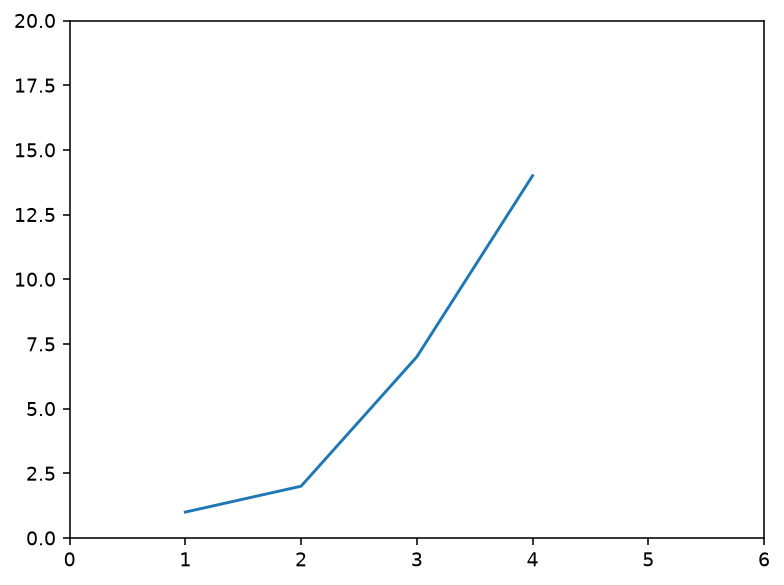
\includegraphics[width=0.94\textwidth]{figures/task3.png}
\end{center}

\clearpage
\section*{\fbox{Task 4}}
\textbf{Question.}
Use Matplotlib to create a figure of your choice in IPython. Paste
the code and figure into the report.

\solution
I plotted the damped oscillation
\[
 y(t)=e^{-0.7t}\cos(2\pi\cdot1.5t),\qquad 0\leq t\leq4.
\]
The oscillation has a frequency of $1.5$ Hz. The dashed curves
$-e^{-0.7t}$ and $e^{-0.7t}$ bound the signal; their magnitudes decrease
as time increases. The code is
\lstinputlisting[language=Python]{snippets/task4.py}
\begin{center}
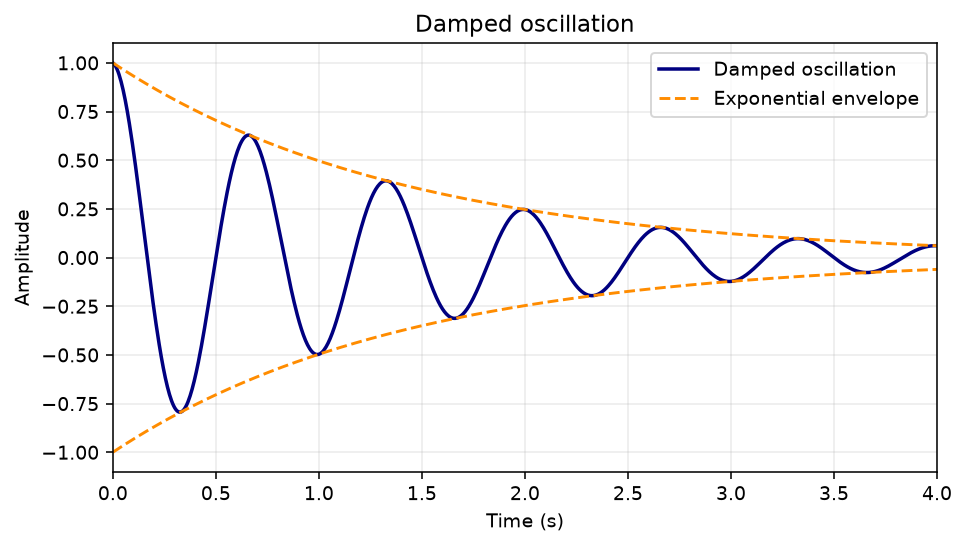
\includegraphics[width=0.96\textwidth]{figures/task4.png}
\end{center}

\clearpage
\section*{\fbox{Task 5}}
\textbf{Question.}
Paste your version control account into the report.

\solution
My GitHub username is \texttt{yunfeixie233}. My profile is
\begin{center}
\url{https://github.com/yunfeixie233}.
\end{center}

\section*{\fbox{Task 6}}
\textbf{Question.}
Start a new project in an IDE of your choice. Commit and push the
project to GitHub as a public project. Paste its link into the report.

\solution
I created the project in Visual Studio Code and pushed it to the
public repository
\begin{center}
\url{https://github.com/yunfeixie233/elec576-assignment0-yunfei-xie}.
\end{center}
The repository contains the executed notebook, Python source files,
figures, and saved results. The README gives the commands to recreate
the notebook and run the numerical checks. Those checks verify array
operations, matrix factorizations, linear-system residuals, Fourier
transforms, and the plotted data.

\begin{thebibliography}{9}
\bibitem{assignment}
ELEC 576 / COMP 576, Fall 2026. \emph{Assignment 0}.
Course handout, due September 15, 2026.
\bibitem{numpy}
NumPy developers. \emph{NumPy for MATLAB users},
``Linear algebra equivalents.''
\url{https://numpy.org/doc/stable/user/numpy-for-matlab-users.html}.
Accessed September 15, 2026.
\bibitem{scipy}
SciPy developers. \emph{SciPy reference guide},
\texttt{scipy.linalg}, \texttt{scipy.sparse.linalg.cg}, and
\texttt{scipy.signal.resample}.
\url{https://docs.scipy.org/doc/scipy/reference/}.
\bibitem{matplotlib}
Matplotlib developers. \emph{Pyplot tutorial}.
\url{https://matplotlib.org/stable/tutorials/pyplot.html}.
\bibitem{stanford}
Stanford CS231n. \emph{Python NumPy tutorial}.
\url{https://cs231n.github.io/python-numpy-tutorial/}.
\bibitem{reference}
Chen Zeng. \emph{Introduction to Deep Learning}, Assignment 0.
\url{https://github.com/ZengChen94/Introduction-to-Deep-Learning}.
Consulted for task coverage and output comparisons.
\end{thebibliography}
\end{document}
